\chapter{Desarollo}

	Dentro de este cap\'itulo se desglosar\'an las etapas que se siguieron en el desarrollo del SII, cada una de estas es parte de la metodolog\'ia de cascada que fue la que se eligi\'o para este desarrollo.

	\section{An\'alisis del sistema}
		Una de las actividades m\'as importantes del Instituto Tecnol\'ogico de Tl\'ahuac es el c\'alculo de indicadores, esto debido a que estos brindan informaci\'on para la mejora de los procesos. El Sistema Integral de Indicadores debe ser capaz de mostrar la informaci\'on requerida por los usuarios de una manera f\'acil, flexible y r\'apida.\\

		La informaci\'on que se requiere del sistema es el seguimiento de los procesos de los diferentes departamentos. Los departamentos a administrar por el sistema son los siguientes:

		\begin{itemize}
			\item Acad\'emico.
			\item Vinculaci\'on.
			\item Planeaci\'on.
			\item Administraci\'on de los recursos.
			\item Calidad.
		\end{itemize}

		Cada uno de ellos requiere obtener informaci\'on espec\'ifica la cual permitir\'a mejorar cada uno de sus procesos.

		El sistema ser\'a capaz de recalcular los indicadores con los cambios que se le presenten a lo largo del periodo declarado, permitiendo con esto tomar decisiones estrat\'egicas para mejorar en caso de que los indicadores sean bajos, o mantener las buenas pr\'acticas en caso de que los indicadores sean los esperados.\\

		Los reportes a configurar dentro del sistema contendr\'an un n\'umero indefinido de c\'alculos, es decir, el n\'umero de datos a calcular es din\'amico permitiendo con esto darle flexibilidad y adaptaci\'on a diferentes circunstancias.\\


		Se necesita que el sistema tenga las siguientes caracter\'isticas:

		\begin{itemize}
			\item \textbf{Configurable:} El sistema debe tener la capacidad de ser configurado de acuerdo a las necesidades de los usuarios.
			\item \textbf{Escalable:} El sistema debe de ser capaz de adaptarse a nuevas funcionalidades y nuevos m\'odulos, esto quiere decir que debe estar listo para que nuevos desarrolladores puedan usar como base este desarrollo para futuras adaptaciones.
			\item \textbf{Amigable:} Es importante que la presentaci\'on del sistema sea agradable para el usuario, debido a que esto mejora la experiencia del mismo permitiendo al usuario tener un ambiente de trabajo agradable.
		\end{itemize}
		
		Con estas tres caracter\'isticas el sistema debe ser capaz de calcular y mostrar las cifras de los indicadores por departamento.

	\section{An\'alisis de requisitos del software}

		Para la realizaci\'on del Sistema Integral de Indicadores se requiere que este se desarrolle en un ambiente Web, esto para permitir que multiples usuarios puedan acceder a estos datos simult\'aneamente.\\

		A lo largo de esta secci\'on se detallaran los distintos tipos de requerimientos necesarios para el desarrollo del sistema.\\

		\subsection{Requerimientos f\'isicos}
			Para el correcto funcionamiento del sistema es necesario contar con el equipo y software  adecuado, del cual hablaremos a continuaci\'on:

			\begin{itemize}
				\item Hardware
					\begin{itemize}
						\item \textbf{Servidor 1:} Equipo con Windows Server 2012 R2 (recomendado) o alg\'un sistema operativo con Windows a 64 bits dedicado para el servidor de base de datos. M\'inimo 4GB de RAM, para su correcto funcionamiento se necesitan 6 GB o m\'as, Procesador x64 a 1.4 GHz, para su correcto funcionamiento procesadores a 2.0 GHz o m\'as. M\'inimo 6GB de disco duro para su instalaci\'on, el tama\~no del disco duro depende a las demandas de espacio al ir almacenando informaci\'on.

						\item \textbf{Servidor 2:} Equipo con Windows Server 2012 R2 (recomendado) o alg\'un sistema operativo con Windows a 64 bits dedicado para el servidor de aplicaci\'on. M\'inimo 2GB de RAM, para su correcto funcionamiento se necesitan 4 GB o m\'as, Procesador x64 a 1.4 GHz, para su correcto funcionamiento procesadores a 2.0 GHz o más. Disco duro de 500GB para almacenamiento de sitios y archivos en servidor.

						\item \textbf{Desarrollo:} Equipo con Windows Server 7 Ultimate a 64 bits dedicado para el desarrollo del sistema, 6GB de RAM o m\'as. Procesador x64 a 1.4 GHz, para su correcto funcionamiento procesadores a 2.0 GHz o m\'as. Disco duro de 500GB para almacenamiento de fuentes y archivos de instalaci\'on.

					\end{itemize}
				\item Software
					\begin{itemize}
						\item Microsoft SQL Server 2012.
						\item IIS Server 8.0 o superior.
						\item Navegador Web (Mozilla Firefox preferentemente)
						\item Microsoft Visual Studio 2013 Test Premium
					\end{itemize}
			\end{itemize}

		El servidor 1 deber\'a tener instalado Microsoft SQL Server 2012 para fungir como servidor de base de datos.\\

		El servidor 1 deber\'a tener instalado IIS Server 8.0 para fungir como servidor de aplicaci\'on y almacenamiento de archivos.\\

		El equipo de desarrollo deber\'a tener instalado Microsoft Visual Studio 2013 Test Premium, Navegador Web adem\'as de IIS Server 8.0 para fungir como ambiente de desarrollo.\\

		\subsection{Interfaces}
		
			El Sistema Integral de Indicadores ser\'a un sistema alimentado de todas las tablas del sistema general. Para esto es necesario establecer los m\'etodos de entrada y salida de datos.\\

			\subsubsection{Entrada de datos}

				Para la entrada de datos es necesario contar con una serie de configuraciones que permitan obtener la informaci\'on de cualquier tabla de la base de datos, esto permitir\'a obtener datos din\'amicos adaptables a las necesidades que tenga en ese momento el usuario.

				Los m\'odulos para realizar la configuraci\'on del sistema son:
				\begin{itemize}
					\item \textbf{Departamentos:} En este m\'odulo se permitir\'a declarar la informaci\'on de los departamentos que se manejar\'an en el SII, los datos requeridos hasta el momento son Id, nombre y descripci\'on.
					\item \textbf{Formulas:} En este m\'odulo se configurar\'an las f\'ormulas que extraer\'an los datos de la base de datos y realizaran los c\'alculos establecidos en estas. Los campos requeridos para configurar una formula son id formula, nombre y la definici\'on de la formula.
					\item \textbf{Colecciones:} Este m\'odulo permite establecer las f\'ormulas que se aplicaran a cada proceso. Las formulas pueden estar en m\'as de un proceso, esto debido a que se puede reutilizar un cálculo de un departamento a otro. Los campos necesarios en este m\'odulo solamente son el id de formula y el id de colecci\'on.
					\item \textbf{Procesos:} En este se definen los datos del periodo dentro de los cuales se necesitan el departamento al que pertenece, numero interno de proceso, descripci\'on, grupo de f\'ormulas a aplicar, fecha de inicio y fin, responsable y unidad de medida.
				\end{itemize}

			\subsubsection{Salida de datos}

				Para la salida de datos se necesita hasta el momento una sola vista en donde se ve el resultado del proceso del periodo de indicadores, esta secci\'on mostrara los siguientes datos:
				\begin{itemize}
					\item \textbf{N\'umero interno de periodo de indicadores:} El n\'umero interno del periodo de indicadores es el identificador \'unico para cada periodo de indicadores.
					\item \textbf{N\'umero consecutivo:} Este se asignar\'a al momento de resolver la formula d\'andole a cada registro del detalle del proceso un identificador.
					\item \textbf{Formula sistema:} Aqu\'i se mostrar\'a la formula tal cual est\'a en el sistema al momento del proceso.
					\item \textbf{Formula pre compilado:} En esta se resuelven las funciones propias del sistema, es decir, las formulas programadas en el sistema, dando como resultado una formula la cual se encuentra lista para ser resuelta por el m\'odulo de f\'ormulas de Microsoft Excel.
					\item \textbf{Resultado:} En este se mostrara el resultado de la formula resuelta por Excel y ser\'a el dato m\'as interesante ya que ser\'a el resultado del indicador.
					De los datos insertados en el sistema, el que requiere de especial atenci\'on es la definici\'on de la formula, esto debido a que si existe alg\'un error en sintaxis al momento de procesar la formulas, esta retornara un valor de 0.
				\end{itemize}

		\subsection{Usuarios y factores humanos}

			El Sistema Integral de Indicadores est\'a pensado para tres tipos de usuarios de usuarios los cuales tendr\'an roles y permisos diferentes. Los usuarios que se podr\'an usar en el sistema son los siguientes:

			\begin{itemize}
				\item Usuario administrador.
				\item Usuario soporte
				\item Usuario consulta
			\end{itemize}

			\subsubsection{Usuario administrador}

				Este usuario tendr\'a permisos para de acceso a todos los m\'odulos teniendo la capacidad de modificar cualquier dato dentro del sistema, adem\'as de tener la capacidad de procesar y reprocesar los periodos de indicadores.\\

				Este usuario debe tener conocimientos de programaci\'on, ya que tendr\'a que programar y modificar funciones para los c\'alculos de indicadores. Ademas deber\'a de tener conocimientos de rastreo de errores y base de datos para poder consultar los errores guardados en el log de base de datos cuando estos se generen. \\

				El usuario de soporte debe hacerse cargo de dar soporte a los tickets reportados referentes a errores l\'ogicos y ajustes de programaci\'on que se requieran seg\'un las necesidades, por lo que este deber\'a tener conocimientos en desarrollo Web con C\# y MVC 4, adem\'as de conocer JQuery y bases de datos con Microsoft SQL Server 2012.\\

			\subsubsection{Usuario soporte}

				Este usuario tendr\'a la capacidad de modificar los datos de los m\'odulos de f\'ormulas y grupos de f\'ormulas con lo cual podr\'a configurar los datos resultantes del proceso de indicadores. Este adem\'as podr\'a tener la capacidad de reprocesar periodos de indicadores con autorizaci\'on de un usuario de soporte.\\

				Este usuario deber\'a de tener conocimientos b\'asicos en programaci\'on para realizar la creaci\'on y modificaci\'on de f\'ormulas de sistema.\\

			\subsubsection{Usuario consulta}
			
				Este usuario es el usuario m\'as limitado del sistema, pues este solamente podr\'a consultar los resultados de los periodos procesados.\\

				Este usuario no necesita conocimientos espec\'ificos ya que su funci\'on es solamente de consulta.

		\subsection{Funcionalidad}

			En esta secci\'on se detalla la funcionalidad que el Sistema Integral de Indicadores tendr\'a.\\

			La funcionalidad del Sistema Integral de Indicadores se ver\'a marcada por 3 etapas muy importantes, las cuales son:
			\begin{itemize}
				\item Configuraci\'on.
				\item Proceso de datos.
				\item Visualizaci\'on de informaci\'on.
			\end{itemize}

			\subsubsection{Configuraci\'on}

				En esta etapa se realizara la configuraci\'on necesaria la cual servir\'a para alimentar el motor de informaci\'on, adem\'as de ser un paso necesario ya que sin \'el no ser\'a posible configurar los par\'ametros de los indicadores.\\

				El proceso de configuraci\'on consta de 3 pasos los cuales se muestran en la figura \ref{fig_ConfiguracionIndicadores}.\\

				\begin{figure}[H]
			        \centering
			        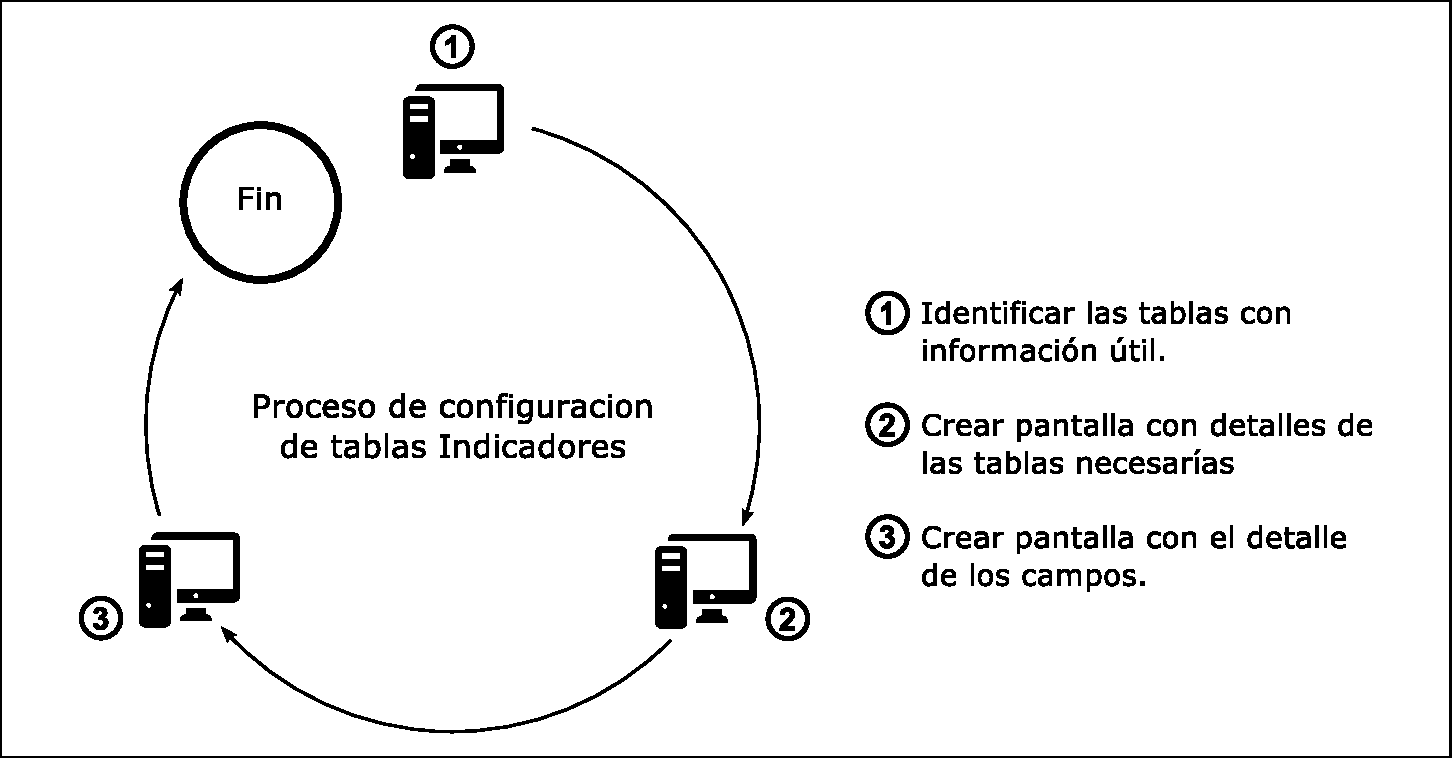
\includegraphics[width=16cm, height=8.5cm]{figuras/ConfiguracionIndicadores}
			        \caption{Diagrama del proceso de configuraci\'on de f\'ormulas de indicadores.}
			        \label{fig_ConfiguracionIndicadores}
			    \end{figure}

		    	\begin{enumerate}[1.]
		    		\item \textbf{Identificar las tablas con informaci\'on \'util.}

		    			El Sistema Integral de Indicadores necesitar\'a contar con la informaci\'on de las tablas del sistema para que \'el pueda generar consultas din\'amicas de informaci\'on, es por esto que se pide identificar las tablas que contienen informaci\'on que sea de utilidad para los fines de los indicadores.
		    			Estas tablas estar\'an disponibles para su consulta y creaci\'on de f\'ormulas permitiendo al usuario la facilidad de consultar cualquier campo que le sea de utilidad.
		    		\item \textbf{Crear pantalla con detalles de las tablas necesarias.}

		    			Este punto consta de realizar el dise\~no de una pantalla  que permita mostrar las tablas en una pantalla para poder ser consultadas y aplicadas directamente a las formulas del sistema.
						Los datos a mostrar en la pantalla son solamente el nombre de la tabla, permitiendo con esto navegar y ubicar los datos de mejor manera. La pantalla de tablas por solicitud del usuario mostrara todas las tablas de la base de datos.
						Estas tablas se mostraran en una lista en el m\'odulo de creaci\'on de f\'ormulas.
					\item \textbf{Crear pantalla con el detalle de los campos.}

						Esta pantalla ser\'a para complementar la pantalla tablas ya que el detalle de los campos de de cada tabla se mostrara en una segunda lista en el m\'odulo de creaci\'on de f\'ormulas, permitiendo con esto tener a la mano todos las herramientas necesarias para el dise\~no de estas.

		    	\end{enumerate}

		    \subsubsection{Proceso de datos}

		    	En este proceso se realizar\'a una de las tareas m\'as delicadas del sistema, ya que es aqu\'i donde se procesar\'a la informaci\'on de los indicadores.\\

				En este proceso se realizaran los c\'alculos de los indicadores, realizando el registro de los datos para tener la informaci\'on organizada seg\'un los datos reales y adem\'as para hacer m\'as eficiente la consulta de informaci\'on.\\

				En este paso se realizarla lo descrito  en la figura \ref{fig_ProcesoIndicador}

				\begin{figure}[H]
			        \centering
			        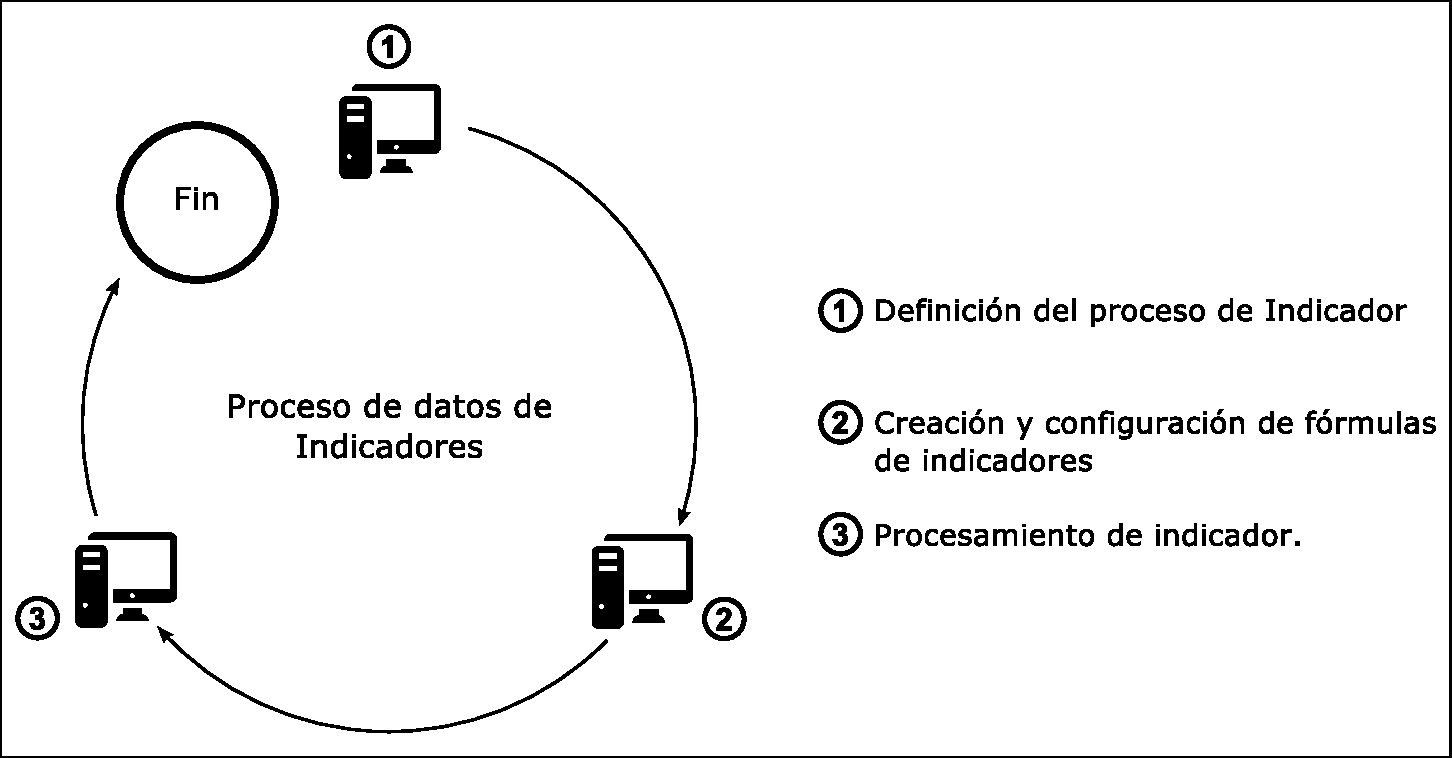
\includegraphics[width=16cm, height=8.5cm]{figuras/ProcesoIndicadores}
			        \caption{Diagrama del proceso de informaci\'on de indicadores.}
			        \label{fig_ProcesoIndicador}
			    \end{figure}

			    La definici\'on de los indicadores es la parte en donde se definen los datos para generar los resultados de los indicadores, el cual se realizara de acuerdo a los lineamientos del Instituto Tecnol\'ogico de Tl\'ahuac el cual establece que la informaci\'on se organizar\'a primeramente por instituci\'on, despu\'es se especificar\'a el departamento al que pertenece el indicador y por \'ultimo se organizar\'an por un rango de fechas especificado manualmente. Este rango de fechas podr\'a ser utilizado en la programaci\'on de las formulas permitiendo filtrar los datos.

			    \begin{enumerate}[1.]
		    		\item \textbf{Definic\'ion del proceso de indicador.}

		    			Este proceso consta de realizar la creaci\'on del proceso de indicador que se desee, para el cual se necesitan los siguientes datos:
		    			\begin{itemize}
		    				\item \textbf{ID instituci\'on:} Este campo contendr\'a el ID de la instituci\'on a la que pertenece el indicador, este campo formar\'a parte de la llave para identificar el indicador.
		    				\item \textbf{Departamento:} Este campo es el n\'umero de departamento.
		    				\item \textbf{N\'umero interno del proceso:} Este campo se autogenerara cuando se crea un nuevo proceso, ya que es \'unico para poder identificar los procesos dentro de todo el sistema.
		    				\item \textbf{Descripci\'on:} Este campo contendr\'a el detalle del contenido del indicador, permitiendo tener un resumen r\'apido del mismo.
		    				\item \textbf{Colecci\'on de f\'ormulas:} Este campo contendr\'a el n\'umero de colecci\'on que se utilizara para realizar el c\'alculo del indicador.
		    				\item \textbf{Fecha inicial:} Fecha de inicio del proceso.
		    				\item \textbf{Fecha final:} Fecha de fin del proceso.
		    				\item \textbf{Responsable:} Este campo es para almacenar el puesto o el nombre del responsable de calcular la informaci\'on de este indicador.
		    				\item \textbf{Unidad de medida:} Especifica la unidad que se utiliza para medir el indicador, este regularmente es un porcentaje.
		    			\end{itemize}

		    		\item \textbf{Configuraci\'on de f\'ormulas de indicadores.}

		    			Este proceso consiste en realizar la configuraci\'on de las f\'ormulas que permitir\'an de manera din\'amica obtener los datos configurados en la misma.

						Para realizar la configuraci\'on de la misma es necesario conocer algunos de los elementos que se pueden utilizar en las mismas los cuales son:
						\begin{itemize}
							\item F\'ormulas definidas en el sistema
							\item F\'ormulas de  Microsoft Excel
						\end{itemize}

						\textbf{F\'ormulas definidas en el sistema:} Esta funcionalidad permite realizar acciones generales basadas en funciones parametrizables, las cuales se podr\'an acceder con la siguiente nomenclatura NOMBRE\_FUNCION (PARAMETRO\_1, PARAMETRO\_2 ... PARAMETRO\_N).

						Con esto la primera capa de resoluci\'on de f\'ormulas nos permite obtener datos procesados en f\'ormulas que se pueden programar en c\'odigo, ampliando la potencia de la resoluci\'on delas mismas.

						\textbf{F\'ormulas de Microsoft Excel:} Esta funcionalidad es el segundo y \'ultimo de los niveles de resoluci\'on de f\'ormulas del sistema de indicadores, ya que al tener los datos obtenidos mediante la resoluci\'on de f\'ormulas de sistema, podemos realizar la resoluci\'on de f\'ormulas de Excel, permitiendo usar la potencia del motor de f\'ormulas de dicho software, y al tener esta posibilidad se pueden obtener los resultados como si estuvi\'eramos en el mismo software.

					\item \textbf{Procesamiento del indicador.}

						Este es el paso final del proceso de datos el cual consiste en realizar el procesamiento de las f\'ormulas y almacenamiento de dichos datos.

						Este proceso se plane\'o con el fin de tener informaci\'on espec\'ifica adem\'as de registrar estos datos en la base de datos para mejorar la eficiencia de la visualizaci\'on de los indicadores. Si este paso no existiera, la resoluci\'on de las f\'ormulas se tendr\'ia que realizar cada que un indicador se visualice generando con esto posibles inconsistencias en la informaci\'on por la adici\'on  nuevos datos, adem\'as de lentitud al momento de usar el sistema.

		    	\end{enumerate}

	\section{Dise\~no del sistema}
		Para el dise\~no del sistema se tomar\'an dos puntos de la metodolog\'ia de cascada los cuales son:
		\begin{itemize}
			\item Estructura de los datos.
			\item Caracterizaci\'on de la interfaz.
		\end{itemize}

		\subsection{Estructura de los datos}

			Para la creaci\'on de la base de datos del Sistema Integral de Indicadores es necesario identificar las entidades principales para poder comenzar con el proceso de dise\~no de la misma. Las entidades que se utilizar\'an en el sistema son:
			\begin{itemize}
				\item Departamentos.
				\item F\'ormulas.
				\item Grupos de f\'ormulas.
				\item Proceso.
			\end{itemize}

			Estas entidades est\'an ligadas con una que ya existe llamada Instituci\'on, la cual tiene la informaci\'on de las instituciones que administra el sistema.\\

			Para relacionar las entidades identificadas se cre\'o un diagrama entidad-relaci\'on como se muestra en la figura \ref{fig_DEntidadRel}.

			\begin{figure}[H]
		        \centering
		        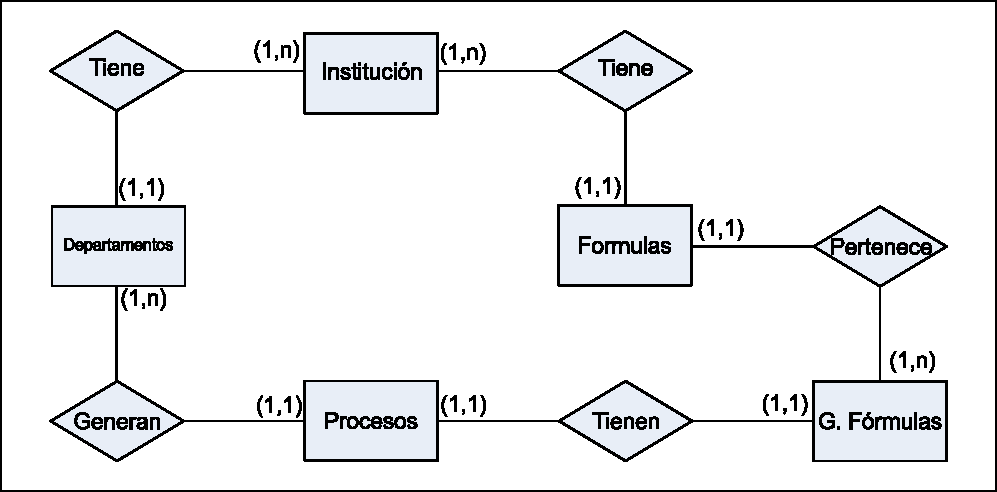
\includegraphics[width=16cm, height=8.5cm]{figuras/DEntidadRel}
		        \caption{Diagrama entidad relaci\'on del sistema de indicadores.}
		        \label{fig_DEntidadRel}
		    \end{figure}

		    \begin{itemize}
		    	\item \textbf{instituci\'on:} Esta entidad es parte del sistema general del Tecnol\'ogico de Tl\'ahuac por lo que solamente haremos referencia a ella para validar la integridad de los datos verificando que los indicadores est\'en ligados a una instituci\'on existente.
		    	\item \textbf{Departamentos:} La entidad departamentos contendr\'a la informaci\'on necesaria de cada departamento como son un identificador, su nombre y descripci\'on. Posteriormente se podr\'an agregar campos para futuras funcionalidades.
		    	\item \textbf{Formulas:} Esta entidad contendr\'a la informaci\'on de las formulas necesaria para ser identificada en el proceso. La informaci\'on que se requiere es la instituci\'on, identificador, nombre y la definici\'on de la f\'ormula. Posteriormente se pueden a\~nadir campos para futuras funcionalidades.
		    	\item \textbf{GFormulas:} Esta entidad est\'a encargada de agrupar las formulas en grupos. Estos grupos ser\'an utilizados para ser procesados en un proceso de indicadores, esta entidad se considerar\'a una entidad compuesta partiendo los datos en encabezado y detalle, permitiendo con esto evitar la redundancia de datos.
		    	\item \textbf{Procesos:} Esta entidad es la parte m\'as importante del sistema de indicadores, pues es en ella donde se almacena el resultado del c\'alculo y avance de los procesos de indicadores. Esta es considerada una entidad compuesta partiendo los datos en encabezado y detalle.
		    \end{itemize}

		    Despu\'es de identificar las entidades compuestas el diagrama sufre algunos cambios, los cuales se muestran en la figura \ref{fig_DEntidadRelComp}.

		    \begin{figure}[H]
		        \centering
		        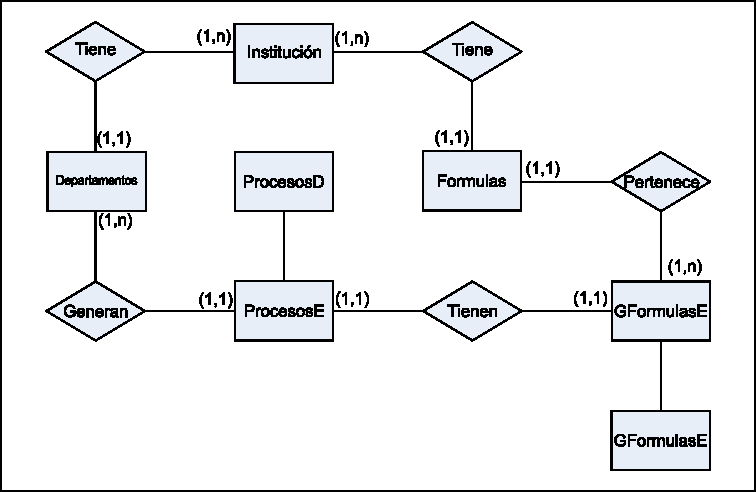
\includegraphics[width=16cm, height=8.5cm]{figuras/DEntidadRelComp}
		        \caption{Diagrama entidad relaci\'on con tablas compuestas del sistema de indicadores.}
		        \label{fig_DEntidadRelComp}
		    \end{figure}

		    \subsubsection{Definici\'on del diccionario de datos del sistema}

		    	De acuerdo a la definici\'on de los datos, se puede generar el diagrama relacional indicando como es que los datos estarán organizados en la base de datos. La figura \ref{fig_DEntidadRelComp} ilustra este diagrama.

		    	\begin{figure}[H]
			        \centering
			        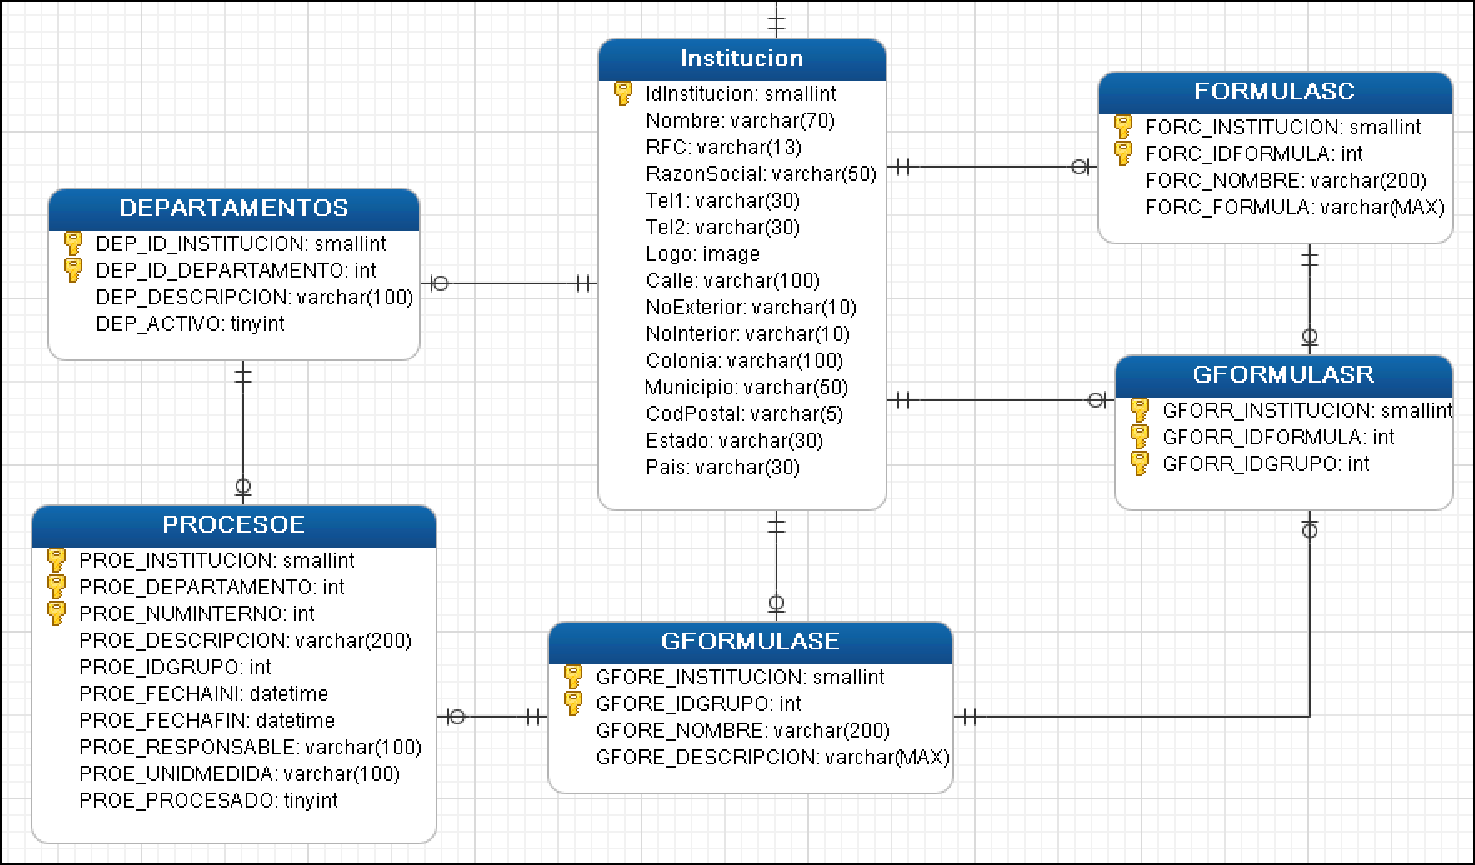
\includegraphics[width=16cm, height=8.5cm]{figuras/Relacional}
			        \caption{Diagrama relaional con campos del sistema de indicadores.}
			        \label{fig_DEntidadRelComp}
			    \end{figure}

		    \subsubsection{Definici\'on del diccionario de datos del sistema}

		    	De acruerdo a los diagramas anteriores, se procede a realizar la definicion del diccionario de datos para la

		    	\begin{table}[H]
				\centering
				\caption{Detalle de los campos de la tabla departamentos.}
				\label{tab_departamentos}
					\begin{tabular}{|l|c|c|c|c|c|c|}
						\hline
						\rowcolor[HTML]{329A9D} 
						\multicolumn{7}{|c|}{\cellcolor[HTML]{329A9D}DEPARTAMENTOS}                                                      \\ \hline
						\rowcolor[HTML]{00D2CB} 
						\multicolumn{1}{|c|}{\cellcolor[HTML]{00D2CB}Nombre} & Tipo     & TipoNativo & Longitud & Precisi\'on & Orden & PK \\ \hline
						DEP\_ACTIVO                                          & tinyint  & tinyint    & 1        & 3         & 4     & No \\ \hline
						DEP\_ID\_INSTITUCION                                 & smallint & smallint   & 2        & 5         & 1     & Si \\ \hline
						DEP\_ID\_DEPARTAMENTO                                & int      & int        & 4        & 10        & 2     & Si \\ \hline
					\end{tabular}
				\end{table}


				\begin{table}[H]
					\centering
					\caption{Detalle de los campos de la tabla formulasc.}
					\label{tab_formulasc}
					\begin{tabular}{|l|c|c|c|c|c|c|}
						\hline
						\rowcolor[HTML]{329A9D} 
						\multicolumn{7}{|c|}{\cellcolor[HTML]{329A9D}FORMULASC}                                                          \\ \hline
						\rowcolor[HTML]{00D2CB} 
						\multicolumn{1}{|c|}{\cellcolor[HTML]{00D2CB}Nombre} & Tipo     & TipoNativo & Longitud & Precisi\'on & Orden & PK \\ \hline
						FORC\_INSTITUCION                                    & smallint & smallint   & 2        & 5         & 1     & Si \\ \hline
						FORC\_IDFORMULA                                      & int      & int        & 4        & 10        & 2     & Si \\ \hline
						FORC\_NOMBRE                                         & varchar  & varchar    & 200      & 200       & 3     & No \\ \hline
						FORC\_FORMULA                                        & varchar  & varchar    & Max      & Max       & 4     & No \\ \hline
					\end{tabular}
				\end{table}

				\begin{table}[H]
					\centering
					\caption{Detalle de los campos de la tabla gformulase.}
					\label{tab_gformulase}
					\begin{tabular}{|l|l|l|l|l|l|l|}
						\hline
						\rowcolor[HTML]{329A9D} 
						\multicolumn{7}{|c|}{\cellcolor[HTML]{329A9D}GFORMULASE}                       \\ \hline
						\rowcolor[HTML]{00D2CB} 
						Nombre             & Tipo     & TipoNativo & Longitud & Precisi\'on & Orden & PK \\ \hline
						GFORE\_INSTITUCION & smallint & smallint   & 2        & 5         & 1     & Si \\ \hline
						GFORE\_IDGRUPO     & int      & int        & 4        & 10        & 2     & Si \\ \hline
						GFORE\_NOMBRE      & varchar  & varchar    & 200      & 200       & 3     & No \\ \hline
						GFORE\_DESCRIPCION & varchar  & varchar    & Max      & Max       & 4     & No \\ \hline
					\end{tabular}
				\end{table}

				\begin{table}[H]
					\centering
					\caption{Detalle de los campos de la tabla gformulasr.}
					\label{tab_gformulasr}
					\begin{tabular}{|c|c|c|c|c|c|c|}
						\hline
						\rowcolor[HTML]{329A9D} 
						\multicolumn{7}{|c|}{\cellcolor[HTML]{329A9D}GFORMULASR}                       \\ \hline
						\rowcolor[HTML]{00D2CB} 
						Nombre             & Tipo     & TipoNativo & Longitud & Precisi\'on & Orden & PK \\ \hline
						GFORR\_INSTITUCION & smallint & smallint   & 2        & 5         & 1     & Si \\ \hline
						GFORR\_IDFORMULA   & int      & int        & 4        & 10        & 2     & Si \\ \hline
						GFORR\_IDGRUPO     & int      & int        & 4        & 10        & 3     & Si \\ \hline
					\end{tabular}
				\end{table}

				\begin{table}[H]
					\centering
					\caption{Detalle de los campos de la tabla procesoe.}
					\label{tab_procesoe}
					\begin{tabular}{|l|c|c|c|c|c|c|}
						\hline
						\rowcolor[HTML]{329A9D} 
						\multicolumn{7}{|c|}{\cellcolor[HTML]{329A9D}PROCESOE}                                                           \\ \hline
						\rowcolor[HTML]{00D2CB} 
						\multicolumn{1}{|c|}{\cellcolor[HTML]{00D2CB}Nombre} & Tipo     & TipoNativo & Longitud & Precisi\'on & Orden & PK \\ \hline
						PROE\_PROCESADO                                      & tinyint  & tinyint    & 1        & 3         & 10    & No \\ \hline
						PROE\_INSTITUCION                                    & smallint & smallint   & 2        & 5         & 1     & Si \\ \hline
						PROE\_DEPARTAMENTO                                   & int      & int        & 4        & 10        & 2     & Si \\ \hline
						PROE\_NUMINTERNO                                     & int      & int        & 4        & 10        & 3     & Si \\ \hline
						PROE\_IDGRUPO                                        & int      & int        & 4        & 10        & 5     & No \\ \hline
						PROE\_FECHAINI                                       & datetime & datetime   & 8        & 23        & 6     & No \\ \hline
						PROE\_FECHAFIN                                       & datetime & datetime   & 8        & 23        & 7     & No \\ \hline
						PROE\_DESCRIPCION                                    & varchar  & varchar    & 200      & 200       & 4     & No \\ \hline
						PROE\_RESPONSABLE                                    & varchar  & varchar    & 100      & 100       & 8     & No \\ \hline
						PROE\_UNIDMEDIDA                                     & varchar  & varchar    & 100      & 100       & 9     & No \\ \hline
					\end{tabular}
				\end{table}

				\begin{table}[H]
					\centering
					\caption{Detalle de los campos de la tabla procesod.}
					\label{tab_procesod}
					\begin{tabular}{|l|c|c|c|c|c|c|}
						\hline
						\rowcolor[HTML]{329A9D} 
						\multicolumn{7}{|c|}{\cellcolor[HTML]{329A9D}PROCESOD}                                                             \\ \hline
						\rowcolor[HTML]{00D2CB} 
						\multicolumn{1}{|c|}{\cellcolor[HTML]{00D2CB}Nombre} & Tipo     & TipoNativo & Longitud & Precisi\'on & Orden & PK \\ \hline
						PROD\_INSTITUCION                                    & smallint & smallint   & 2        & 5           & 1     & Si \\ \hline
						PROD\_NUMINTERNO                                     & int      & int        & 4        & 10          & 2     & Si \\ \hline
						PROD\_CONSECUTIVO                                    & int      & int        & 4        & 10          & 3     & Si \\ \hline
						PROD\_FORMULASIS                                     & varchar  & varchar    & Max      & Max         & 4     & No \\ \hline
						PROD\_FORMULAPRE                                     & varchar  & varchar    & Max      & Max         & 5     & No \\ \hline
						PROD\_FORMULARES                                     & varchar  & varchar    & Max      & Max         & 6     & No \\ \hline
					\end{tabular}
				\end{table}

				Con esto la definici\'on de los datos queda completa, permitiendo tener los argumentos suficientes para la descripci\'on de las interfaces.





	\section{Caracterizaci\'on de la interfaz}

		Para la definici\'on de la funcionalidad de la interfaz se tomaran en cuenta los siguientes requerimientos generales:
		\begin{itemize}
			\item Los tipos de dato de los componentes de entrada de las interfaces estar\'an definidos de acuerdo al tipo de dato nativo en la BD, esto para mejorar la experiencia del usuario.
			\item Todas las entradas de datos se mostrar\'an en ventanas emergentes.
			\item La visualizaci\'on de los datos se har\'a en una tabla para mejorar la accesibilidad de los datos
			\item Las acciones propias a los registros serán colocadas a la derecha de la tabla, estas no tendr\'an t\'itulo de encabezado.
			\item Se crearan los botones de navegaci\'on del sistema en la parte superior derecha de las tablas, estas acciones ser\'an determinadas por m\'odulo.
			\item En el caso de que no existan registros para mostrar en el m\'odulo, deber\'a de mostrar un mensaje descriptivo a la situaci\'on, dejando invisibles los encabezados de la tabla propia del m\'odulo.
		\end{itemize}

		En el caso de algunos m\'odulos, se deber\'an de tomar algunas consideraciones especiales las cuales se describe continuaci\'on:

		\begin{itemize}
			\item \textbf{Colecciones:} En el caso de este formulario se deber\'a agregar una columna que muestre un bot\'on, este bot\'on re direccionara al formulario DetalleColecciones.
			\item \textbf{DetalleColecciones:} Este formulario contara \'unicamente con las funciones de agregar y eliminar, se deshabilita la funci\'on de actualizar ya que aqu\'i no se pueden modificar las formulas si no solo agregarlas o eliminarlas. 

			La funcionalidad de agregar se mostrara en una ventana emergente la cual tendr\'a \'unicamente una lista multi-selecci\'on que mostrara las f\'ormulas que est\'an disponibles para ser agregadas a la colecci\'on.
			\item \textbf{Proceso:} Este dormulario mostrara los registros del encabezado de los procesos con las siguientes funcionalidades.
			\begin{itemize}
				\item \textbf{Crear:} Esta funcionalidad permitir\'a crear un nuevo proceso.
				\item \textbf{Actualizar:} Esta funcionalidad permite actualizar los datos del periodo. Cuando se realiza esta acci\'on es importante mencionar que el periodo puede que necesite reprocesarse, ya que los datos como las fechas de inicio y fin o el n\'umero de colecci\'on de f\'ormulas afectan directamente en el resultado.
				\item \textbf{Eliminar:} Esta funcionalidad permite eliminar un proceso. Es importante destacar que al eliminar un proceso se eliminaran tanto los registros en el encabezado y el detalle.
				\item \textbf{Procesar:} Esta funcionalidad ejecuta la resoluci\'on de f\'ormulas del sistema guardando los resultados en el detalle del proceso.
				\item \textbf{Detalle:} Esta funcionalidad muestra los registros que se encuentran en el detalle del proceso. Este formulario es solo de consulta por lo que no se tendr\'a ninguna funcionalidad.
			\end{itemize}
		\end{itemize}



	\section{Programaci\'on}

		Dentro de los puntos destacables para la codificaci\'on de este proyecto, se detectaron procesos los cuales, debido a su constante repetici\'on, se hizo c\'odigo reutilizable que permitiera manejar estos casos.\\
		
		Para dar una soluci\'on a este problema, se utiliz\'o el framework que el Instituto Tecnol\'ogico de Tláhuac está desarrollando, el cual cuenta con muchas tareas programadas que pueden sernos de gran utilidad.\\

		\subsection{Manejo de interfaces de mensajes emergentes}

			Los menajes emergentes dentro del sistema son una de las tareas que a nivel de programaci\'on requieren realizar la repetici\'on de c\'odigo, haciendo con esto que este se vuelva ilegible y muy dif\'icil de entender. Para solucionar este punto se cre\'o una clase dentro del proyecto de las utiler\'ias del Framework del Instituto Tecnol\'ogico de Tl\'ahuac la cual se encarga de realizar el manejo de la creaci\'on del c\'odigo que contendr\'a el cuerpo de este mensaje.\\

			Las acciones que soporta esta clase son las siguientes:
			\begin{itemize}
				\item Creaci\'on de ventana emergente para creaci\'on, actualizaci\'on y eliminaci\'on de datos del sistema.
				\item Ejecuci\'on de acciones de creaci\'on, actualizaci\'on y eliminaci\'on de informaci\'on.
				\item Acciones especiales de m\'odulos.
			\end{itemize}

			Cada una de estas acciones est\'a delimitada a usarse de acuerdo al nombre del m\'odulo que se ejecuten, es decir, si se quisiera la ventana emergente para la creaci\'on de un nuevo registro en el m\'odulo de departamentos sea visible, basta con indicar que se requiere el alta del formulario junto con el nombre del departamento.\\

			Las acciones a ejecutar dentro de cada uno de estas ventanas emergentes se encuentra tambi\'en en esta clase, la cual realiza las actividades necesarias para realizar la actualizaci\'on o eliminaci\'on de estos modulo.


